\documentclass{jlreq}
\usepackage{amsmath,ascmac,amssymb,mathtools,siunitx,inputenc, amsthm}

\usepackage{graphicx}
\usepackage[svgnames]{xcolor}
\usepackage{float,subcaption,tikz}

%% tcolorbox %%
\usepackage{tcolorbox}

\tcbuselibrary{raster,skins,theorems,breakable}
\tcbset{
    breakable,
    coltitle=black,
    colbacktitle=white,
    boxrule=2pt,
    colback=white,
    fonttitle=\bfseries,
}

\newcounter{theorem}[section]

\newtcolorbox[auto counter, number within = section]{definition}[1][]{
    colframe=RoyalBlue,
    title=定義 \thetcbcounter.~#1
}
\newtcolorbox[auto counter, number within = section]{theorem}[1][]{
    colframe=DarkCyan,
    title=定理 \thetcbcounter.~#1
}
\newtcolorbox[auto counter, number within = section]{lemma}[1][]{
    colframe=DarkCyan,
    title=補題 \thetcbcounter.~#1
}
\newtcolorbox[auto counter, number within = section]{corollary}[1][]{
    colframe=DarkCyan,
    title=系 \thetcbcounter.~#1
}
\newtcolorbox[auto counter, number within = section]{remark}[1][]{
    colframe=OliveDrab,
    title=Remark \thetcbcounter.~#1
}
\newtcolorbox[auto counter, number within = section]{observation}[1][]{
    colframe=OliveDrab,
    title=Observation \thetcbcounter.~#1
}


\usepackage{graphicx}
\usepackage[svgnames]{xcolor}
\usepackage{float,subcaption,tikz}
\usepackage{hyperref}
\hypersetup{
    unicode,
    setpagesize=false,
    bookmarksnumbered=true,
    bookmarksopen=true,
    colorlinks=true,
    linkcolor=DarkCyan,
    citecolor=Chocolate,
    urlcolor=Chocolate
}

\newcommand\Includegraphics[2][]{\vcenter{\hbox{\includegraphics[#1]{#2}}}}
\graphicspath{{../images/}}

\usepackage[backend=biber]{biblatex}
\addbibresource{../ref/ref.bib}
\usepackage{unicmd}
\usepackage{subfiles}

\begin{document}
\title{Verlinde公式の証明}
\author{政岡凜太郎}
\maketitle

以下ではCFTとしてミニマル模型を仮定する。
またプライマリー場と言ったときはVirasoroプライマリー場を指す。

\section{OPEとフュージョン}

\begin{align}
    ϕ_i(z)ϕ_i(0) = ∑_{k, Y} C_{ij}^{k, Y}z^{h_k-h_i-h_j+|Y|}ℒ_{-Y}ϕ_k(0)
\end{align}
\begin{align}
    ϕ_i(z)| h_j ⟩ = ∑_{k, Y} C_{ij}^{k, Y}z^{h_k-h_i-h_j+|Y|}L_{-Y}| h_k ⟩
\end{align}
\begin{align}
    L_n ϕ_i(z)| h_j ⟩
    &
    = [L_n, ϕ_i(z)]| h_j ⟩ \∅
    &
    = (z^{n+1}∂_z + (n+1)h_i)ϕ_i(z)| h_j ⟩ \∅
    &
    = ∑_k z^{h_k-h_i-h_j}∑_{Y} z^{|Y|+n} (h_k+nh_i-h_j-|Y|)C_{ij}^{k, Y}L_{-Y}| h_k ⟩ \∅
    &
    = ∑_k z^{h_k-h_i-h_j} ∑_Y z^{|Y|} C_{ij}^{k, Y}[L_n, L_{-Y}]| h_k ⟩.
\end{align}
\begin{align}
    ∑_{|Y|=N} (h_k+nh_i-h_j-N)C_{ij}^{k, Y}L_{-Y}| h_k ⟩
    = ∑_{|Y|=N+n} C_{ij}^{k, Y}[L_n, L_{-Y}]| h_k ⟩
\end{align}
$n=1$, $N=0$とすると、
\begin{align}
    (h_k+h_i-h_j)C_{ij}^{k, 0}| h_k ⟩ = C_{ij}^{k, 1}[L_1, L_{-1}]| h_k ⟩ = C_{ij}^{k, 1} 2h_k| h_k ⟩
\end{align}
を得る。したがって、
\begin{align}
    ÷{C_{ij}^{k,1}}{C_{ij}^{k, 0}} = ÷{h_k+h_i-h_j}{2h_k}
\end{align}
が分かる。
\begin{align}
    L_Y ϕ_i(z)| h_j ⟩
    = [L_Y, ϕ_i(z)] | h_j ⟩ 
    % = ∑_k z^{h_k-h_i-h_j} ∑_{Y'} z^{|Y|+|Y'|}f(h_i, h_k-h_i-h_j+|Y'|, Y)C_{i,j}^{k, Y}L_{-Y}| h_k ⟩ \∅
    % &
    = ∑_k z^{h_k-h_i-h_j} ∑_{Y'} z^{|Y'|} C_{ij}^{k, Y}[L_Y, L_{-Y}]| h_k ⟩.
\end{align}
したがって、$|Y|=N$の係数$C_{i,j}^{k, Y}$を決めるために$p(N)$個の拘束条件を用いることができるため、$C_{ij}^{k, Y}$も$C_{i,j}^{k, 0}$によって表すことができる。
\section{トーラス上のCFT}
トーラス上のCFTにおける基本的な知識を復習する。
トーラスは複素平面$ℂ$に以下の同一視を入れることで得られる。
\begin{align}
    z \sim z + 1,␣
    z \sim z + τ
\end{align}
ここで$τ ∈ ℂ$はモジュラーパラメーターと呼ばれる。
格子$Λ$を$Λ ≔ \{n+mτ\mid n,m∈ℤ\}$によって定義すると、このトーラスは$ℂ/Λ$と書くことができる。
ここで、$Λ$を不変に保つような$τ$の変換をモジュラー変換という。
具体的には以下の1次分数変換がモジュラー変換の一般形である。
\begin{align}
    τ ↦ ÷{a+bτ}{c+dτ},␣ ad-bc=1.
    \label{modular transformation}
\end{align}
モジュラー変換のなす群をモジュラー群と呼ぶ。モジュラー群は$\SL(2,ℤ)/ℤ_2$に同型である。
この群は以下の2つの元から生成される。
\begin{align}
    T: τ ↦ τ+1,␣
    S: τ ↦ -÷1{τ}.
\end{align}

トーラス上のCFTの分配関数は
\begin{align}
    Z(τ) = \Tr(q^{L₀-c/24}\_q^{\_L₀-c/24}),␣
    q = 𝑒^{2π𝑖}
\end{align}
である。プライマリー場$i$から生成される共形族への射影を$Π_i$とおくと、指標は
\begin{align}
    χ_i(q) ≔ \Tr(Π_iq^{L₀-c/24}),␣
    q = e^{2πiτ}
\end{align}
と定義される。
ここで
ここで$\Tr$は正則部分のHilbert空間についてのものである。
すると分配関数は
\begin{align}
    Z(τ) = ∑_{i, j}ℳ_{ij} χ_i(q)\_χ_j(\_q)
\end{align}
と表すことができる。ここで$ℳ_{ij}$はCFTに存在する共形ウェイトが$(h_i, \_h_j)$となるようなプライマリー場の個数を表す。

分配関数はモジュラー変換に対して不変である。すなわち
\begin{align}
    Z(τ) = Z(τ+1) = Z( -÷1{τ} )
\end{align}
が成り立つ。では指標についてはどうだろう。
$T$変換については指標の変換性は簡単に求まる。具体的には、
\begin{align}
    χ_i(q) ↦ \Tr(Π_ie^{2π𝑖(τ+1)(L₀-c/24)})
    = e^{2π𝑖(h_i-c/24)}χ_i(q)
\end{align}
となる。
次に、$S$変換についてだが、以下の事実を用いよう。
\begin{lemma}
    $\{f_i(z)\}_{i=1}^N$, $\{f'_i(z)\}_{i=1}^N$, $\{g_i(z)\}_{i=1}^N$, $\{g'_i(z)\}_{i=1}^N$を線形独立な正則関数の組とする。
    これらが
    \begin{align}
        ∑_{i=1}^N f_i(z)\_{f}'_i(\_z) = ∑_{i=1}^M g_i(z)\_{g}'_i(\_z)
        \label{crossing like equation}
    \end{align}
    を満たすならば、$f_i(z) = ∑_j M_{ij}g_j(z)$, $\_{f}'_i(\_z) = ∑_j M'_{ij} \_{g}'_i(\_z)$と表せる。ここで$M_{ij}, M'_{ij}$は可逆な行列である。
\end{lemma}

\begin{proof}
    (\ref{crossing like equation})を微分していくと、
    \begin{align}
        ∑_{i=1}^N f_i^{(n)}(z)\_{f}'_i(\_z) = ∑_{i=1}^M g_i^{(n)}(z)\_{g}'_i(\_z)
    \end{align}
    を得る。よって、Wronskianを$W^f_{ni}(z) = f_i^{(n)}(z)$, $W^g_{ni}(z) = g_i^{(n)}(z)$によって定義すると、
    \begin{align}
        W^f(z)\→{f}'(\_z) = W^g(z)\→{g}'(\_z).
    \end{align}
    ここで$\→{f}', \→{g}'$は$\_f'_i, \_g'_i$を成分にもつベクトルである。
    $\{f_i(z)\}_{i=1}^N$の線形独立性から$\det W^f(z₀) ≠ 0$となる$z₀$が存在するので、$\→{f}'(\_z) = (W^f)^{-1}(z₀)W^g(z₀)\→{g}'(\_z) ≕ M'\→{g}'$と書ける。
    同様に$\det W^g(z₁) ≠ 0$となる$z₁$も存在するので、$\→{g}'(\_z) = (W^g)^{-1}(z₁)W^f(z₁)\→{f}'(\_z) = (M')^{-1}\→{f}'(\_z)$となる。
    したがって線形変換$M'$の可逆性が分かる。$\→f, \→g$についても同様。
\end{proof}

この補題を用いると、分配関数のモジュラー不変性
\begin{align}
    Z(τ) = ∑_{i,j}ℳ_{i,j}χ_i(q)\overline{χ_j(q)}
    = ∑_{i,j}ℳ_{i,j}χ_i(\~q)\overline{χ_j(\~q)} = Z( -÷1{τ} ),␣
    \~q = e^{-2π𝑖/τ}
\end{align}
から、指標の$S$変換による変換性を
\begin{align}
    χ_i(\~q) = ∑_{j}S_{ij}χ_j(q),␣
    \~q = e^{-2πi/τ}
\end{align}
のように線形変換として書くことができる。
この$S_{ij}$をモジュラー$S$行列と呼ぶ。

\section{Verlinde公式}
Verlindeはフュージョン係数$N_{ij}^k$とモジュラー$S$行列の間に成り立つ以下の驚くべき関係式を予想した。
\begin{theorem}[Verlinde公式]
    \begin{align}
        N_{ij}^k = ∑_l ÷{S_{il}S_{jl}(S^{-1})_{kl}}{S_{0l}}
        \label{Verlinde formula}
    \end{align}
\end{theorem}
この公式にはいくつかの証明があるようだが、Verlindeの原論文の議論に沿った証明を紹介する。
\footnote{
    Verlindeの原論文では(\ref{Verlinde formula})の左辺がフュージョン係数として満たすべき性質のいくつかを満たすことを示しているが、それがフュージョン係数に完全に一致することは示していない。
    Verlinde公式を実際に証明したのはMoore--Seibergである。
}
記号はYellow bookに従う。

まず指標$χ_j$に対し、トーラス上の2点にそれぞれプライマリー場$ϕ_i(z)$とその共役$ϕ_{i^*}(w)$を挿入することができる。
適切に規格化をし、$z → w$とすれば、もとの指標が再現される:
\begin{align}
    χ_j = \lim_{z→w}(z-w)^{2h_i}ℱ^{i,i^*}_j(z-w).
\end{align}
トーラスの非自明な2つのサイクルをそれぞれ$𝖺$ (空間方向), $𝖻$(時間方向)と書く。
\begin{figure}[H]
    \centering
    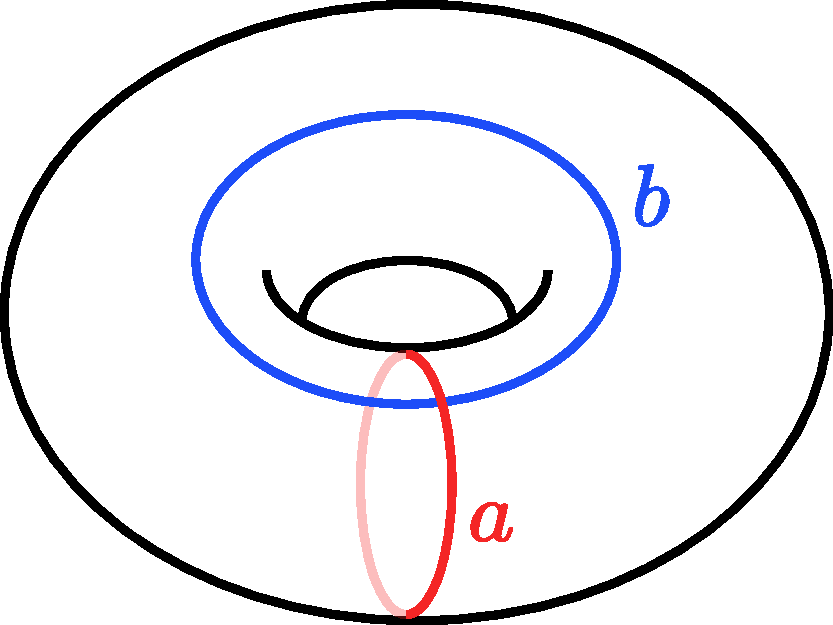
\includegraphics[width=0.2\hsize]{two_cycles}
\end{figure}
$χ_i$に対して$ϕ_i(z), ϕ_{i^*}(w)$を挿入したあと, $ϕ_{i^*}(w)$を非自明なサイクルに沿って連続的に動かしていき、一周してから$ϕ_i(z), ϕ_{i^*}(w)$を接近させて対消滅させる、という操作を考える。
ここで$ϕ_{i^*}(w)$を連続的に動かす、というのは$ℱ^{i,i^*}_j(z-w)$を$w$について解析接続することを指す。
この操作を$ϕ_i(𝖺)$または$ϕ_i(𝖻)$という記号で表そう。
これは場のように書いているが、実際には指標がなす空間に作用する線形変換である。

$ϕ_i(𝖺)$の方は簡単である。
指標$χ_j$について、射影$Π_j$は$𝖺$に沿って挿入されていることから、挿入した場を射影$Π_j$に触れずに$𝖺$に沿って動かすことができる。
\begin{figure}[H]
    \centering
    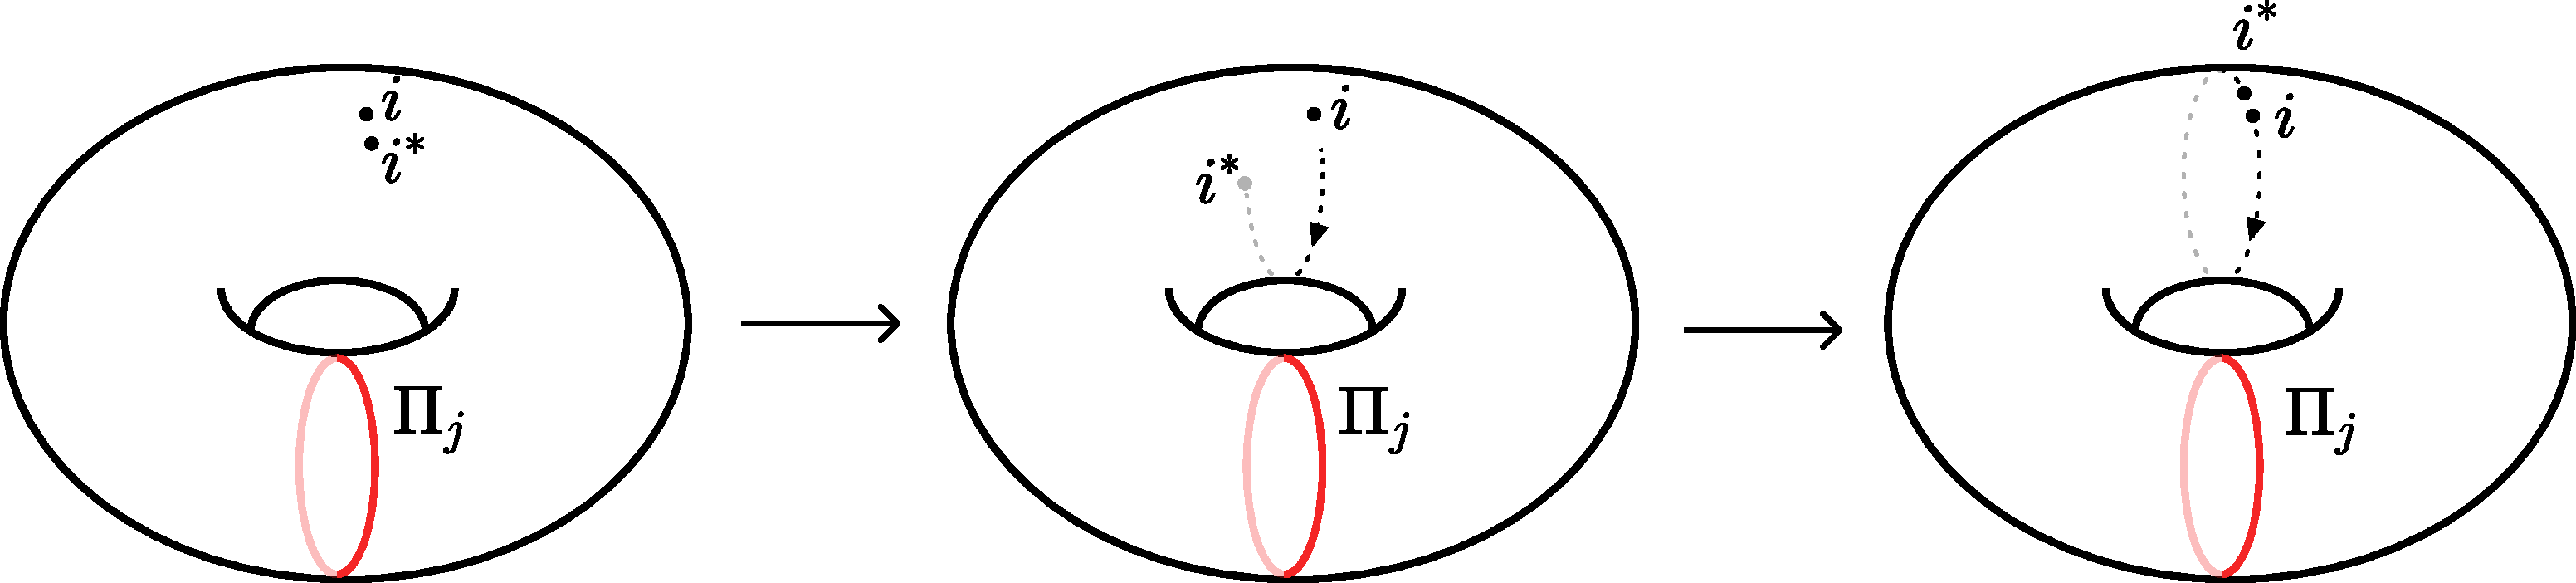
\includegraphics[width=0.8\hsize]{phi_a}
\end{figure}
したがって$ϕ_i(𝖺)$の操作によって$Π_j$に影響が及ぶことがないため、$ϕ_i(𝖺)$は指標$χ_i$が張る1次元空間に作用する。
すなわち定数$γ^{(j)}_i$によって
\begin{align}
    ϕ_i(𝖺)χ_j = γ_i^{(j)}χ_j
\end{align}
と表せる。

問題となるのは$ϕ_i(𝖻)$の方である。この場合$ϕ_{i^*}(w)$を動かしていくと射影$Π_j$と衝突するため、フュージョンによって他の指標$χ_k$が現れることが予想される。
結論から述べると、なんと厳密に
\begin{align}
    ϕ_i(𝖻)χ_j = ∑_k N_{ij}^k χ_k
    \label{action of phi_b}
\end{align}
となる。
まずこの式を証明できれば、Verlinde公式が従うことを示す。
$ϕ_i(𝖺)$と$ϕ_i(𝖻)$はモジュラー変換でつながるため、
\begin{align}
    ϕ_i(𝖻) = Sϕ_i(𝖺)S^{-1}
\end{align}
が成り立つ。$ϕ_i(𝖺)$が対角行列であったことを思い出すとこの式は$ϕ_i(b)$がモジュラー$S$行列によって同時対角化されることを意味している。
(\ref{action of phi_b})を認めれば、このことはフュージョン係数$N_{ij}^k$が$S$によって対角化されることを意味する:
\begin{align}
    N_{ij}^k = ∑_l S_{il}γ_j^{(l)}(S^{-1})_{kl}.
\end{align}
ここで$N_{0j}^k = δ_j^k$を代入すると、
\begin{align}
    δ_j^k = ∑_l S_{0l}γ_j^{(l)}(S^{-1})_{kl}.
\end{align}
両辺に右から$∑_k S_{kl}$を掛けると、
\begin{align}
    S_{jl} = S_{0l}γ_j^{(l)}.
\end{align}
よって、Verlinde公式が従う:
\begin{align}
    N_{ij}^k = ∑_l ÷{S_{il}S_{jl}(S^{-1})_{kl}}{S_{0l}}
\end{align}

さて、問題の式(\ref{action of phi_b})を示そう。
まず$ϕ_i(𝖻)$は以下のようなダイアグラムによって表すことができる。
\begin{figure}[H]
    \centering
    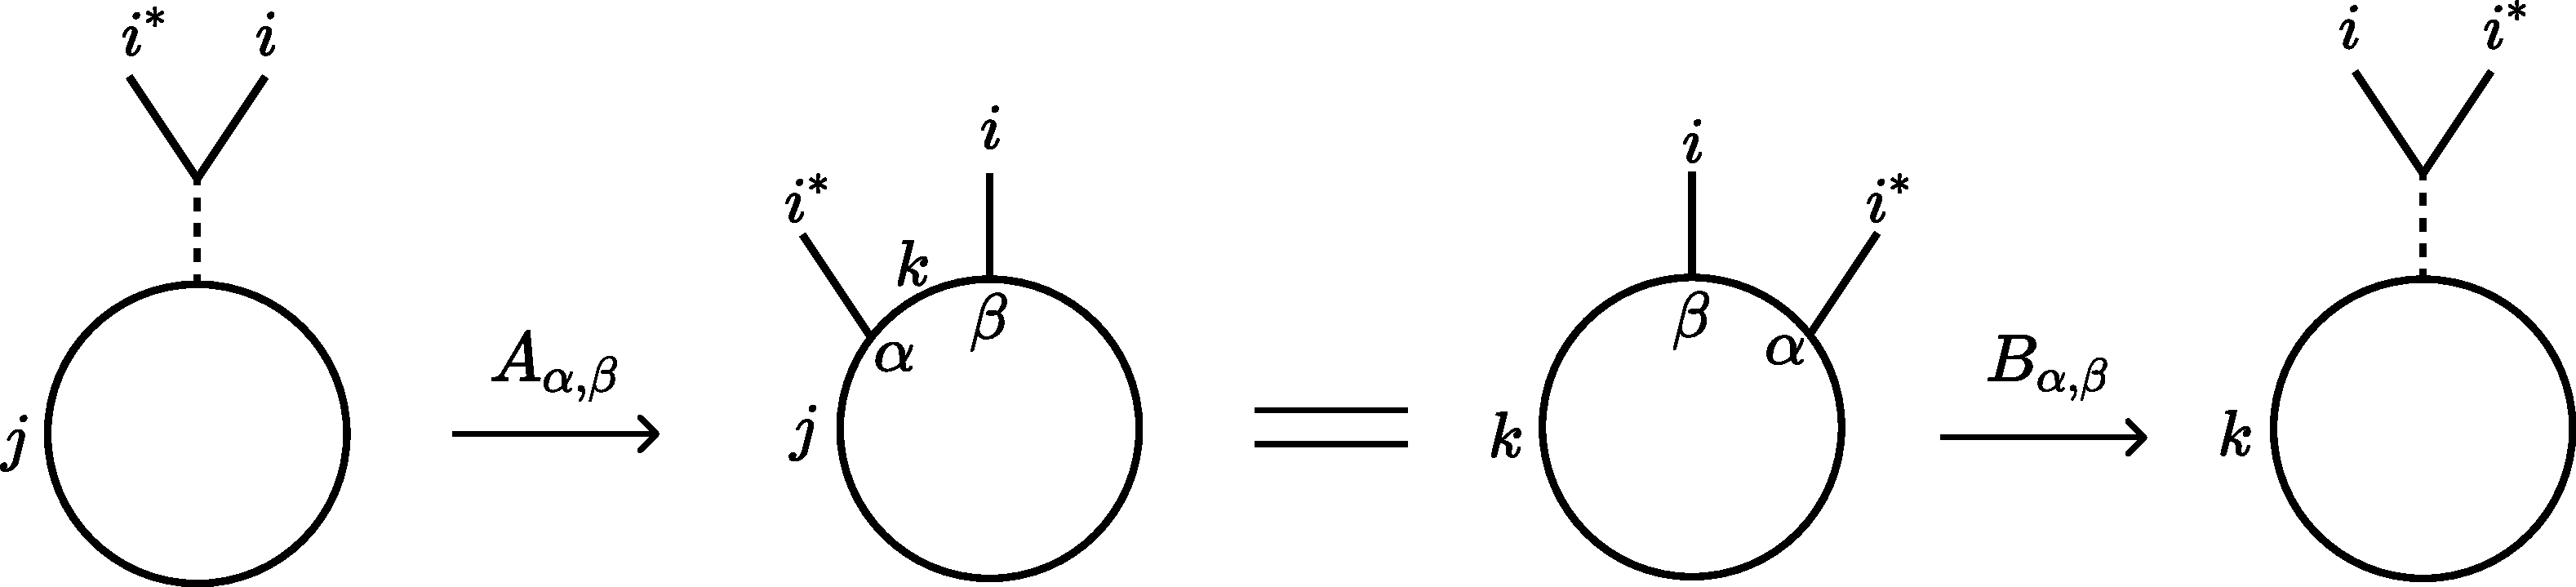
\includegraphics[width=0.8\hsize]{phi_a chi_j}
\end{figure}
ここで$A_{α, β}, B_{α, β}$は適切な$F$行列によって記述されるべきものだが、添字をたくさん書くのが面倒なのでこのように書いている。
また添字に関しての和は省いている。
ただし、これが$ϕ_i(𝖻)$を表すのではなく、$ϕ_i(𝖻)$の定数倍を表している。
規格化定数を決定するために、$j=0$とする。
するとダイアグラムは
\begin{figure}[H]
    \centering
    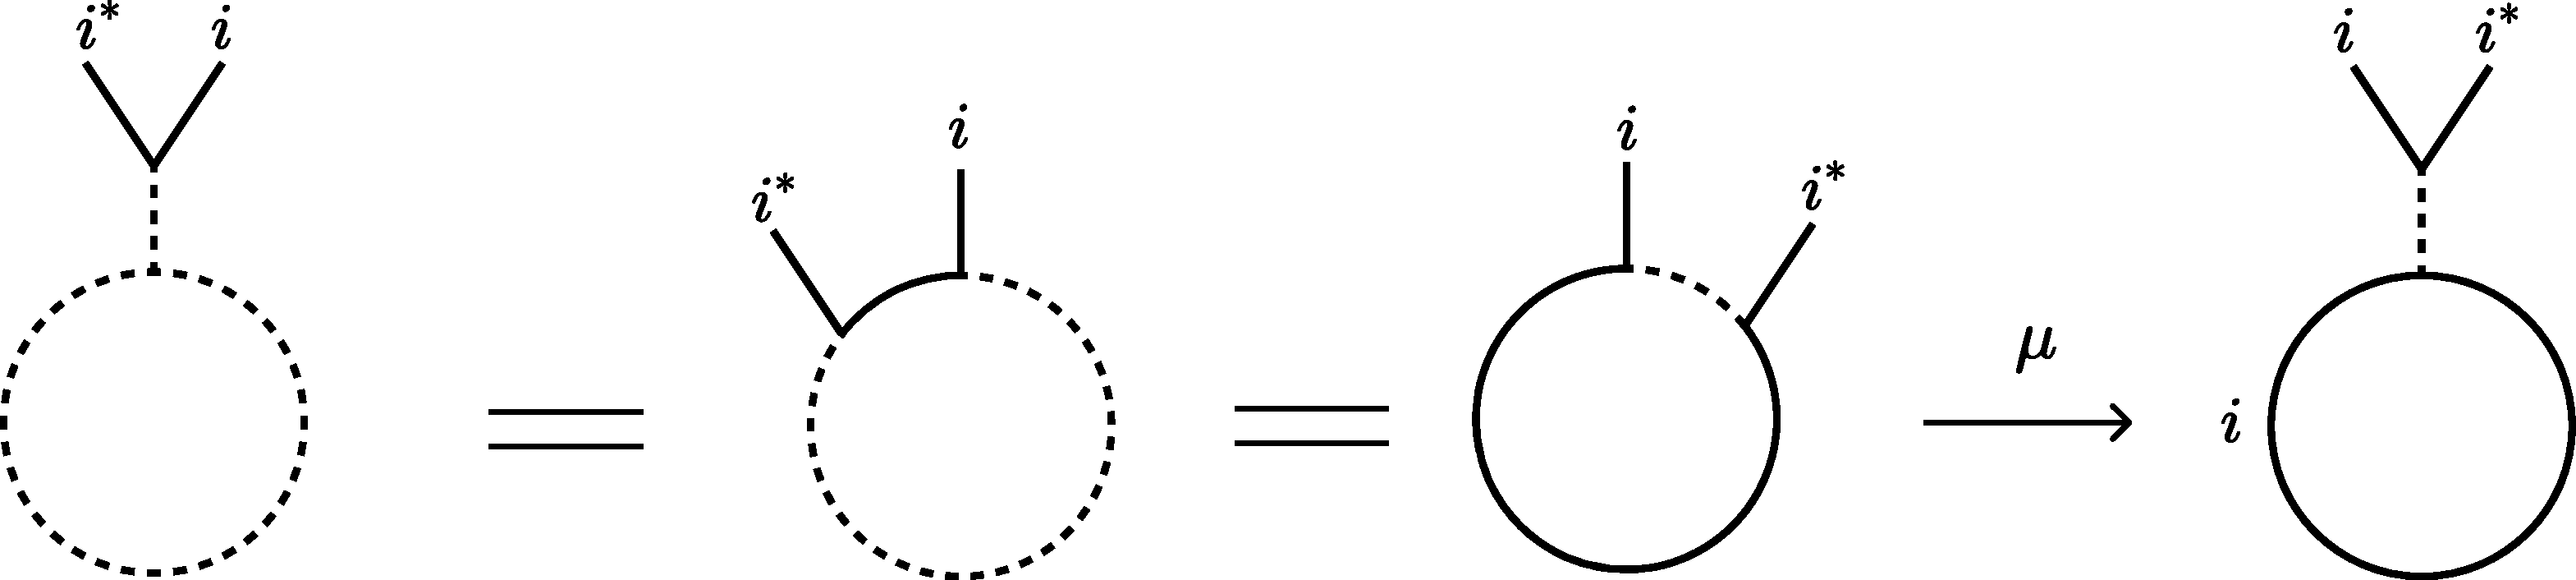
\includegraphics[width=0.8\hsize]{phi_a chi_0}
\end{figure}
となる。$μ$も$F$行列から定義されるが、中間チャネルが全て真空なため、結局定数になる。
この操作は$μϕ_i(b)$に等しいから、
\begin{align}
    ϕ_i(𝖻)χ_j = ÷1{μ} ∑_{α, β} A_{α, β}B_{α, β} χ_j
    \label{phi_b by A and B}
\end{align}
を得る。
さらに、以下のpentagon equationを考える。
\begin{figure}[H]
    \centering
    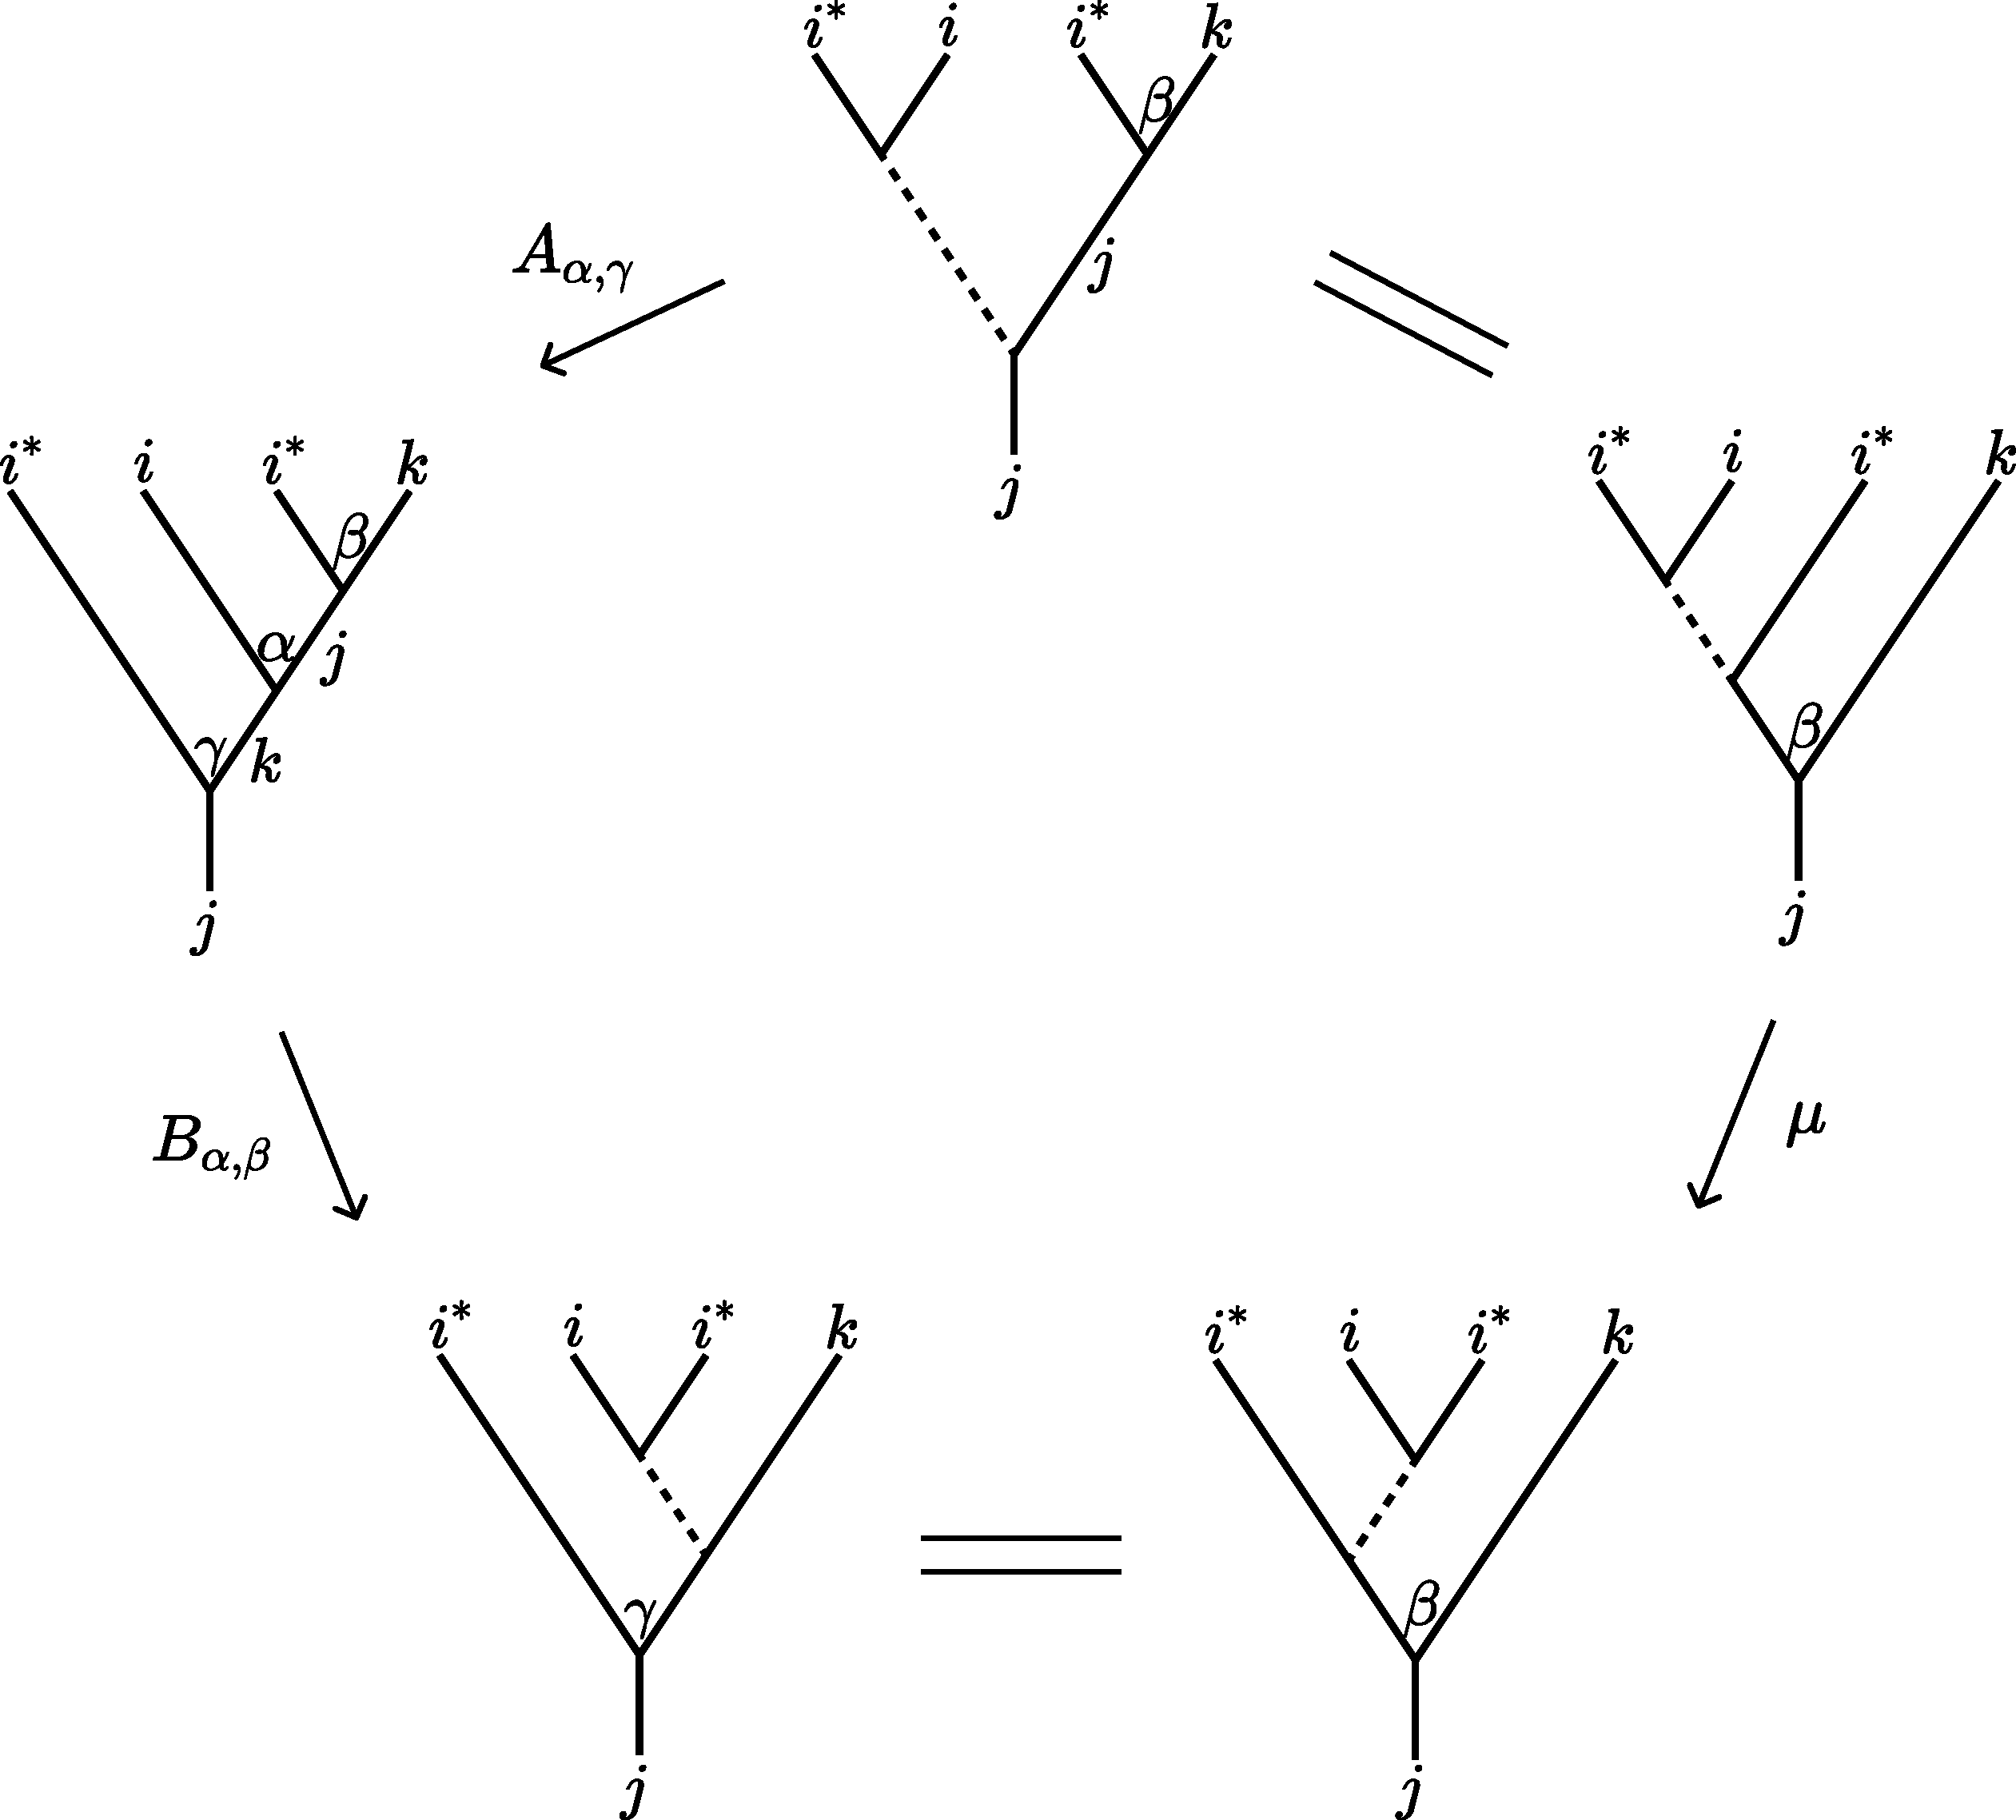
\includegraphics[width=0.7\hsize]{pentagon}
\end{figure}
すると
\begin{align}
    ∑_{α, γ}A_{α,γ}B_{α,β} = ∑_{α}A_{α, β}B_{α, β}
    = μ
\end{align}
を得る。ここで、$β=γ$となることを用いた。
$β=1,…,N_{ij}^k$について和をとると、
\begin{align}
    ∑_{α, β}A_{α, β}B_{α, β} = μN_{ij}^k.
\end{align}
この式を(\ref{phi_b by A and B})に代入することで、(\ref{action of phi_b})が示される。
\end{document}